
% Default to the notebook output style

    


% Inherit from the specified cell style.




    
\documentclass[11pt]{article}

    
    
    \usepackage[T1]{fontenc}
    % Nicer default font (+ math font) than Computer Modern for most use cases
    \usepackage{mathpazo}

    % Basic figure setup, for now with no caption control since it's done
    % automatically by Pandoc (which extracts ![](path) syntax from Markdown).
    \usepackage{graphicx}
    % We will generate all images so they have a width \maxwidth. This means
    % that they will get their normal width if they fit onto the page, but
    % are scaled down if they would overflow the margins.
    \makeatletter
    \def\maxwidth{\ifdim\Gin@nat@width>\linewidth\linewidth
    \else\Gin@nat@width\fi}
    \makeatother
    \let\Oldincludegraphics\includegraphics
    % Set max figure width to be 80% of text width, for now hardcoded.
    \renewcommand{\includegraphics}[1]{\Oldincludegraphics[width=.8\maxwidth]{#1}}
    % Ensure that by default, figures have no caption (until we provide a
    % proper Figure object with a Caption API and a way to capture that
    % in the conversion process - todo).
    \usepackage{caption}
    \DeclareCaptionLabelFormat{nolabel}{}
    \captionsetup{labelformat=nolabel}

    \usepackage{adjustbox} % Used to constrain images to a maximum size 
    \usepackage{xcolor} % Allow colors to be defined
    \usepackage{enumerate} % Needed for markdown enumerations to work
    \usepackage{geometry} % Used to adjust the document margins
    \usepackage{amsmath} % Equations
    \usepackage{amssymb} % Equations
    \usepackage{textcomp} % defines textquotesingle
    % Hack from http://tex.stackexchange.com/a/47451/13684:
    \AtBeginDocument{%
        \def\PYZsq{\textquotesingle}% Upright quotes in Pygmentized code
    }
    \usepackage{upquote} % Upright quotes for verbatim code
    \usepackage{eurosym} % defines \euro
    \usepackage[mathletters]{ucs} % Extended unicode (utf-8) support
    \usepackage[utf8x]{inputenc} % Allow utf-8 characters in the tex document
    \usepackage{fancyvrb} % verbatim replacement that allows latex
    \usepackage{grffile} % extends the file name processing of package graphics 
                         % to support a larger range 
    % The hyperref package gives us a pdf with properly built
    % internal navigation ('pdf bookmarks' for the table of contents,
    % internal cross-reference links, web links for URLs, etc.)
    \usepackage{hyperref}
    \usepackage{longtable} % longtable support required by pandoc >1.10
    \usepackage{booktabs}  % table support for pandoc > 1.12.2
    \usepackage[inline]{enumitem} % IRkernel/repr support (it uses the enumerate* environment)
    \usepackage[normalem]{ulem} % ulem is needed to support strikethroughs (\sout)
                                % normalem makes italics be italics, not underlines
    

    
    
    % Colors for the hyperref package
    \definecolor{urlcolor}{rgb}{0,.145,.698}
    \definecolor{linkcolor}{rgb}{.71,0.21,0.01}
    \definecolor{citecolor}{rgb}{.12,.54,.11}

    % ANSI colors
    \definecolor{ansi-black}{HTML}{3E424D}
    \definecolor{ansi-black-intense}{HTML}{282C36}
    \definecolor{ansi-red}{HTML}{E75C58}
    \definecolor{ansi-red-intense}{HTML}{B22B31}
    \definecolor{ansi-green}{HTML}{00A250}
    \definecolor{ansi-green-intense}{HTML}{007427}
    \definecolor{ansi-yellow}{HTML}{DDB62B}
    \definecolor{ansi-yellow-intense}{HTML}{B27D12}
    \definecolor{ansi-blue}{HTML}{208FFB}
    \definecolor{ansi-blue-intense}{HTML}{0065CA}
    \definecolor{ansi-magenta}{HTML}{D160C4}
    \definecolor{ansi-magenta-intense}{HTML}{A03196}
    \definecolor{ansi-cyan}{HTML}{60C6C8}
    \definecolor{ansi-cyan-intense}{HTML}{258F8F}
    \definecolor{ansi-white}{HTML}{C5C1B4}
    \definecolor{ansi-white-intense}{HTML}{A1A6B2}

    % commands and environments needed by pandoc snippets
    % extracted from the output of `pandoc -s`
    \providecommand{\tightlist}{%
      \setlength{\itemsep}{0pt}\setlength{\parskip}{0pt}}
    \DefineVerbatimEnvironment{Highlighting}{Verbatim}{commandchars=\\\{\}}
    % Add ',fontsize=\small' for more characters per line
    \newenvironment{Shaded}{}{}
    \newcommand{\KeywordTok}[1]{\textcolor[rgb]{0.00,0.44,0.13}{\textbf{{#1}}}}
    \newcommand{\DataTypeTok}[1]{\textcolor[rgb]{0.56,0.13,0.00}{{#1}}}
    \newcommand{\DecValTok}[1]{\textcolor[rgb]{0.25,0.63,0.44}{{#1}}}
    \newcommand{\BaseNTok}[1]{\textcolor[rgb]{0.25,0.63,0.44}{{#1}}}
    \newcommand{\FloatTok}[1]{\textcolor[rgb]{0.25,0.63,0.44}{{#1}}}
    \newcommand{\CharTok}[1]{\textcolor[rgb]{0.25,0.44,0.63}{{#1}}}
    \newcommand{\StringTok}[1]{\textcolor[rgb]{0.25,0.44,0.63}{{#1}}}
    \newcommand{\CommentTok}[1]{\textcolor[rgb]{0.38,0.63,0.69}{\textit{{#1}}}}
    \newcommand{\OtherTok}[1]{\textcolor[rgb]{0.00,0.44,0.13}{{#1}}}
    \newcommand{\AlertTok}[1]{\textcolor[rgb]{1.00,0.00,0.00}{\textbf{{#1}}}}
    \newcommand{\FunctionTok}[1]{\textcolor[rgb]{0.02,0.16,0.49}{{#1}}}
    \newcommand{\RegionMarkerTok}[1]{{#1}}
    \newcommand{\ErrorTok}[1]{\textcolor[rgb]{1.00,0.00,0.00}{\textbf{{#1}}}}
    \newcommand{\NormalTok}[1]{{#1}}
    
    % Additional commands for more recent versions of Pandoc
    \newcommand{\ConstantTok}[1]{\textcolor[rgb]{0.53,0.00,0.00}{{#1}}}
    \newcommand{\SpecialCharTok}[1]{\textcolor[rgb]{0.25,0.44,0.63}{{#1}}}
    \newcommand{\VerbatimStringTok}[1]{\textcolor[rgb]{0.25,0.44,0.63}{{#1}}}
    \newcommand{\SpecialStringTok}[1]{\textcolor[rgb]{0.73,0.40,0.53}{{#1}}}
    \newcommand{\ImportTok}[1]{{#1}}
    \newcommand{\DocumentationTok}[1]{\textcolor[rgb]{0.73,0.13,0.13}{\textit{{#1}}}}
    \newcommand{\AnnotationTok}[1]{\textcolor[rgb]{0.38,0.63,0.69}{\textbf{\textit{{#1}}}}}
    \newcommand{\CommentVarTok}[1]{\textcolor[rgb]{0.38,0.63,0.69}{\textbf{\textit{{#1}}}}}
    \newcommand{\VariableTok}[1]{\textcolor[rgb]{0.10,0.09,0.49}{{#1}}}
    \newcommand{\ControlFlowTok}[1]{\textcolor[rgb]{0.00,0.44,0.13}{\textbf{{#1}}}}
    \newcommand{\OperatorTok}[1]{\textcolor[rgb]{0.40,0.40,0.40}{{#1}}}
    \newcommand{\BuiltInTok}[1]{{#1}}
    \newcommand{\ExtensionTok}[1]{{#1}}
    \newcommand{\PreprocessorTok}[1]{\textcolor[rgb]{0.74,0.48,0.00}{{#1}}}
    \newcommand{\AttributeTok}[1]{\textcolor[rgb]{0.49,0.56,0.16}{{#1}}}
    \newcommand{\InformationTok}[1]{\textcolor[rgb]{0.38,0.63,0.69}{\textbf{\textit{{#1}}}}}
    \newcommand{\WarningTok}[1]{\textcolor[rgb]{0.38,0.63,0.69}{\textbf{\textit{{#1}}}}}
    
    
    % Define a nice break command that doesn't care if a line doesn't already
    % exist.
    \def\br{\hspace*{\fill} \\* }
    % Math Jax compatability definitions
    \def\gt{>}
    \def\lt{<}
    % Document parameters
    \title{Bachelor's}
    
    
    

    % Pygments definitions
    
\makeatletter
\def\PY@reset{\let\PY@it=\relax \let\PY@bf=\relax%
    \let\PY@ul=\relax \let\PY@tc=\relax%
    \let\PY@bc=\relax \let\PY@ff=\relax}
\def\PY@tok#1{\csname PY@tok@#1\endcsname}
\def\PY@toks#1+{\ifx\relax#1\empty\else%
    \PY@tok{#1}\expandafter\PY@toks\fi}
\def\PY@do#1{\PY@bc{\PY@tc{\PY@ul{%
    \PY@it{\PY@bf{\PY@ff{#1}}}}}}}
\def\PY#1#2{\PY@reset\PY@toks#1+\relax+\PY@do{#2}}

\expandafter\def\csname PY@tok@w\endcsname{\def\PY@tc##1{\textcolor[rgb]{0.73,0.73,0.73}{##1}}}
\expandafter\def\csname PY@tok@c\endcsname{\let\PY@it=\textit\def\PY@tc##1{\textcolor[rgb]{0.25,0.50,0.50}{##1}}}
\expandafter\def\csname PY@tok@cp\endcsname{\def\PY@tc##1{\textcolor[rgb]{0.74,0.48,0.00}{##1}}}
\expandafter\def\csname PY@tok@k\endcsname{\let\PY@bf=\textbf\def\PY@tc##1{\textcolor[rgb]{0.00,0.50,0.00}{##1}}}
\expandafter\def\csname PY@tok@kp\endcsname{\def\PY@tc##1{\textcolor[rgb]{0.00,0.50,0.00}{##1}}}
\expandafter\def\csname PY@tok@kt\endcsname{\def\PY@tc##1{\textcolor[rgb]{0.69,0.00,0.25}{##1}}}
\expandafter\def\csname PY@tok@o\endcsname{\def\PY@tc##1{\textcolor[rgb]{0.40,0.40,0.40}{##1}}}
\expandafter\def\csname PY@tok@ow\endcsname{\let\PY@bf=\textbf\def\PY@tc##1{\textcolor[rgb]{0.67,0.13,1.00}{##1}}}
\expandafter\def\csname PY@tok@nb\endcsname{\def\PY@tc##1{\textcolor[rgb]{0.00,0.50,0.00}{##1}}}
\expandafter\def\csname PY@tok@nf\endcsname{\def\PY@tc##1{\textcolor[rgb]{0.00,0.00,1.00}{##1}}}
\expandafter\def\csname PY@tok@nc\endcsname{\let\PY@bf=\textbf\def\PY@tc##1{\textcolor[rgb]{0.00,0.00,1.00}{##1}}}
\expandafter\def\csname PY@tok@nn\endcsname{\let\PY@bf=\textbf\def\PY@tc##1{\textcolor[rgb]{0.00,0.00,1.00}{##1}}}
\expandafter\def\csname PY@tok@ne\endcsname{\let\PY@bf=\textbf\def\PY@tc##1{\textcolor[rgb]{0.82,0.25,0.23}{##1}}}
\expandafter\def\csname PY@tok@nv\endcsname{\def\PY@tc##1{\textcolor[rgb]{0.10,0.09,0.49}{##1}}}
\expandafter\def\csname PY@tok@no\endcsname{\def\PY@tc##1{\textcolor[rgb]{0.53,0.00,0.00}{##1}}}
\expandafter\def\csname PY@tok@nl\endcsname{\def\PY@tc##1{\textcolor[rgb]{0.63,0.63,0.00}{##1}}}
\expandafter\def\csname PY@tok@ni\endcsname{\let\PY@bf=\textbf\def\PY@tc##1{\textcolor[rgb]{0.60,0.60,0.60}{##1}}}
\expandafter\def\csname PY@tok@na\endcsname{\def\PY@tc##1{\textcolor[rgb]{0.49,0.56,0.16}{##1}}}
\expandafter\def\csname PY@tok@nt\endcsname{\let\PY@bf=\textbf\def\PY@tc##1{\textcolor[rgb]{0.00,0.50,0.00}{##1}}}
\expandafter\def\csname PY@tok@nd\endcsname{\def\PY@tc##1{\textcolor[rgb]{0.67,0.13,1.00}{##1}}}
\expandafter\def\csname PY@tok@s\endcsname{\def\PY@tc##1{\textcolor[rgb]{0.73,0.13,0.13}{##1}}}
\expandafter\def\csname PY@tok@sd\endcsname{\let\PY@it=\textit\def\PY@tc##1{\textcolor[rgb]{0.73,0.13,0.13}{##1}}}
\expandafter\def\csname PY@tok@si\endcsname{\let\PY@bf=\textbf\def\PY@tc##1{\textcolor[rgb]{0.73,0.40,0.53}{##1}}}
\expandafter\def\csname PY@tok@se\endcsname{\let\PY@bf=\textbf\def\PY@tc##1{\textcolor[rgb]{0.73,0.40,0.13}{##1}}}
\expandafter\def\csname PY@tok@sr\endcsname{\def\PY@tc##1{\textcolor[rgb]{0.73,0.40,0.53}{##1}}}
\expandafter\def\csname PY@tok@ss\endcsname{\def\PY@tc##1{\textcolor[rgb]{0.10,0.09,0.49}{##1}}}
\expandafter\def\csname PY@tok@sx\endcsname{\def\PY@tc##1{\textcolor[rgb]{0.00,0.50,0.00}{##1}}}
\expandafter\def\csname PY@tok@m\endcsname{\def\PY@tc##1{\textcolor[rgb]{0.40,0.40,0.40}{##1}}}
\expandafter\def\csname PY@tok@gh\endcsname{\let\PY@bf=\textbf\def\PY@tc##1{\textcolor[rgb]{0.00,0.00,0.50}{##1}}}
\expandafter\def\csname PY@tok@gu\endcsname{\let\PY@bf=\textbf\def\PY@tc##1{\textcolor[rgb]{0.50,0.00,0.50}{##1}}}
\expandafter\def\csname PY@tok@gd\endcsname{\def\PY@tc##1{\textcolor[rgb]{0.63,0.00,0.00}{##1}}}
\expandafter\def\csname PY@tok@gi\endcsname{\def\PY@tc##1{\textcolor[rgb]{0.00,0.63,0.00}{##1}}}
\expandafter\def\csname PY@tok@gr\endcsname{\def\PY@tc##1{\textcolor[rgb]{1.00,0.00,0.00}{##1}}}
\expandafter\def\csname PY@tok@ge\endcsname{\let\PY@it=\textit}
\expandafter\def\csname PY@tok@gs\endcsname{\let\PY@bf=\textbf}
\expandafter\def\csname PY@tok@gp\endcsname{\let\PY@bf=\textbf\def\PY@tc##1{\textcolor[rgb]{0.00,0.00,0.50}{##1}}}
\expandafter\def\csname PY@tok@go\endcsname{\def\PY@tc##1{\textcolor[rgb]{0.53,0.53,0.53}{##1}}}
\expandafter\def\csname PY@tok@gt\endcsname{\def\PY@tc##1{\textcolor[rgb]{0.00,0.27,0.87}{##1}}}
\expandafter\def\csname PY@tok@err\endcsname{\def\PY@bc##1{\setlength{\fboxsep}{0pt}\fcolorbox[rgb]{1.00,0.00,0.00}{1,1,1}{\strut ##1}}}
\expandafter\def\csname PY@tok@kc\endcsname{\let\PY@bf=\textbf\def\PY@tc##1{\textcolor[rgb]{0.00,0.50,0.00}{##1}}}
\expandafter\def\csname PY@tok@kd\endcsname{\let\PY@bf=\textbf\def\PY@tc##1{\textcolor[rgb]{0.00,0.50,0.00}{##1}}}
\expandafter\def\csname PY@tok@kn\endcsname{\let\PY@bf=\textbf\def\PY@tc##1{\textcolor[rgb]{0.00,0.50,0.00}{##1}}}
\expandafter\def\csname PY@tok@kr\endcsname{\let\PY@bf=\textbf\def\PY@tc##1{\textcolor[rgb]{0.00,0.50,0.00}{##1}}}
\expandafter\def\csname PY@tok@bp\endcsname{\def\PY@tc##1{\textcolor[rgb]{0.00,0.50,0.00}{##1}}}
\expandafter\def\csname PY@tok@fm\endcsname{\def\PY@tc##1{\textcolor[rgb]{0.00,0.00,1.00}{##1}}}
\expandafter\def\csname PY@tok@vc\endcsname{\def\PY@tc##1{\textcolor[rgb]{0.10,0.09,0.49}{##1}}}
\expandafter\def\csname PY@tok@vg\endcsname{\def\PY@tc##1{\textcolor[rgb]{0.10,0.09,0.49}{##1}}}
\expandafter\def\csname PY@tok@vi\endcsname{\def\PY@tc##1{\textcolor[rgb]{0.10,0.09,0.49}{##1}}}
\expandafter\def\csname PY@tok@vm\endcsname{\def\PY@tc##1{\textcolor[rgb]{0.10,0.09,0.49}{##1}}}
\expandafter\def\csname PY@tok@sa\endcsname{\def\PY@tc##1{\textcolor[rgb]{0.73,0.13,0.13}{##1}}}
\expandafter\def\csname PY@tok@sb\endcsname{\def\PY@tc##1{\textcolor[rgb]{0.73,0.13,0.13}{##1}}}
\expandafter\def\csname PY@tok@sc\endcsname{\def\PY@tc##1{\textcolor[rgb]{0.73,0.13,0.13}{##1}}}
\expandafter\def\csname PY@tok@dl\endcsname{\def\PY@tc##1{\textcolor[rgb]{0.73,0.13,0.13}{##1}}}
\expandafter\def\csname PY@tok@s2\endcsname{\def\PY@tc##1{\textcolor[rgb]{0.73,0.13,0.13}{##1}}}
\expandafter\def\csname PY@tok@sh\endcsname{\def\PY@tc##1{\textcolor[rgb]{0.73,0.13,0.13}{##1}}}
\expandafter\def\csname PY@tok@s1\endcsname{\def\PY@tc##1{\textcolor[rgb]{0.73,0.13,0.13}{##1}}}
\expandafter\def\csname PY@tok@mb\endcsname{\def\PY@tc##1{\textcolor[rgb]{0.40,0.40,0.40}{##1}}}
\expandafter\def\csname PY@tok@mf\endcsname{\def\PY@tc##1{\textcolor[rgb]{0.40,0.40,0.40}{##1}}}
\expandafter\def\csname PY@tok@mh\endcsname{\def\PY@tc##1{\textcolor[rgb]{0.40,0.40,0.40}{##1}}}
\expandafter\def\csname PY@tok@mi\endcsname{\def\PY@tc##1{\textcolor[rgb]{0.40,0.40,0.40}{##1}}}
\expandafter\def\csname PY@tok@il\endcsname{\def\PY@tc##1{\textcolor[rgb]{0.40,0.40,0.40}{##1}}}
\expandafter\def\csname PY@tok@mo\endcsname{\def\PY@tc##1{\textcolor[rgb]{0.40,0.40,0.40}{##1}}}
\expandafter\def\csname PY@tok@ch\endcsname{\let\PY@it=\textit\def\PY@tc##1{\textcolor[rgb]{0.25,0.50,0.50}{##1}}}
\expandafter\def\csname PY@tok@cm\endcsname{\let\PY@it=\textit\def\PY@tc##1{\textcolor[rgb]{0.25,0.50,0.50}{##1}}}
\expandafter\def\csname PY@tok@cpf\endcsname{\let\PY@it=\textit\def\PY@tc##1{\textcolor[rgb]{0.25,0.50,0.50}{##1}}}
\expandafter\def\csname PY@tok@c1\endcsname{\let\PY@it=\textit\def\PY@tc##1{\textcolor[rgb]{0.25,0.50,0.50}{##1}}}
\expandafter\def\csname PY@tok@cs\endcsname{\let\PY@it=\textit\def\PY@tc##1{\textcolor[rgb]{0.25,0.50,0.50}{##1}}}

\def\PYZbs{\char`\\}
\def\PYZus{\char`\_}
\def\PYZob{\char`\{}
\def\PYZcb{\char`\}}
\def\PYZca{\char`\^}
\def\PYZam{\char`\&}
\def\PYZlt{\char`\<}
\def\PYZgt{\char`\>}
\def\PYZsh{\char`\#}
\def\PYZpc{\char`\%}
\def\PYZdl{\char`\$}
\def\PYZhy{\char`\-}
\def\PYZsq{\char`\'}
\def\PYZdq{\char`\"}
\def\PYZti{\char`\~}
% for compatibility with earlier versions
\def\PYZat{@}
\def\PYZlb{[}
\def\PYZrb{]}
\makeatother


    % Exact colors from NB
    \definecolor{incolor}{rgb}{0.0, 0.0, 0.5}
    \definecolor{outcolor}{rgb}{0.545, 0.0, 0.0}



    
    % Prevent overflowing lines due to hard-to-break entities
    \sloppy 
    % Setup hyperref package
    \hypersetup{
      breaklinks=true,  % so long urls are correctly broken across lines
      colorlinks=true,
      urlcolor=urlcolor,
      linkcolor=linkcolor,
      citecolor=citecolor,
      }
    % Slightly bigger margins than the latex defaults
    
    \geometry{verbose,tmargin=1in,bmargin=1in,lmargin=1in,rmargin=1in}
    
    

    \begin{document}
    
    
    \maketitle
    
    

    
    \hypertarget{automated-nn-tuning}{%
\section{Automated NN Tuning}\label{automated-nn-tuning}}

\textbf{Autor: }Aiordăchioaei Marius \textbar{} \textbf{Îndrumător:
}Suciu Mihai

    \hypertarget{table-of-contents}{%
\section{Table of contents}\label{table-of-contents}}

\begin{enumerate}
\def\labelenumi{\arabic{enumi}.}
\item
  Intro

  \begin{enumerate}
  \def\labelenumii{\arabic{enumii}.}
  \item
    Abstract
  \item
    Motivation
  \end{enumerate}
\item
  Core concepts

  \begin{enumerate}
  \def\labelenumii{\arabic{enumii}.}
  \setcounter{enumii}{2}
  \item
    Genetic Programming
  \item
    Artificial Neural Networks
  \item
    Convolutional Neural Networks
  \item
    Integration
  \item
    Classical Problems
  \end{enumerate}
\item
  Aplicability

  \begin{enumerate}
  \def\labelenumii{\arabic{enumii}.}
  \setcounter{enumii}{7}
  \item
    Algorithm Overview
  \item
    Web Interface
  \item
    Software Design
  \end{enumerate}
\item
  Feasability and Impact Analysis

  \begin{enumerate}
  \def\labelenumii{\arabic{enumii}.}
  \setcounter{enumii}{10}
  \item
    Performance indicators
  \item
    Efficiency indicators
  \item
    Digit recognition
  \item
    Sentiment analysis
  \end{enumerate}
\end{enumerate}

    \hypertarget{intro}{%
\section{1. Intro}\label{intro}}

    \hypertarget{a.-abstract}{%
\subsection{A. Abstract}\label{a.-abstract}}

With the Artificial Neural Networks becoming more and more popular and
used across all domains, a common problem with designing an eficient one
is the tuning of the so-called ``Hyperparameters''.

An empirical aproach that addresses this problem is through manual trial
and error. This aproach is (most of the time) inefficient and over the
hand in almost all the possible ways. Another aproach is doing R\&D
(Research and Development) on other scientifical publications and
finding problems simmilar to ours' that have been solved.

The aim of this paper is to demonstrate the feasibility of using a third
aproach, automating the process of tweaking the parameters using methods
such as Evolutionary Algorithms to find the right Neural Network, fit
for a specific domain problem.

The process of finding the right Evolutionary Algorithm was all trial
and error, with each step documented. Based on some ad-hoc metrics, the
algorithm could be brought to a state in which is better for the
specific task that are performing.

\hypertarget{keywords}{%
\subsubsection{Keywords:}\label{keywords}}

Evolutionary algorithm, genetic algorithm, genetic programming,
artificial neural network, hyperparameter, brute-force, fitness, natural
selection

    \hypertarget{b.-motivation}{%
\subsection{B. Motivation}\label{b.-motivation}}

    This concept is nothing new. It was researched before and proved to be
efficient, and the idea of automating a trial-and-error job can cross
anyone's mind at some point.

The work will foscus more on the Evolutionary part rather than on the
Neural Network part. It will also contain a detailed feasibility study
of the found solution and testing it with some classical Machine
Learning problems

    \hypertarget{core-concepts}{%
\section{2. Core concepts}\label{core-concepts}}

In the following lines we are going to explain the two
concepts/techniques used in our case study, as well as the integration
between the two

    \hypertarget{a.-genetic-programming}{%
\subsection{A. Genetic programming}\label{a.-genetic-programming}}

Genetic programming and Evolutionary Algorithms reffer to a technique of
solving problems which solutions are in a wide space of possible
solutions. Imagine a solution space which grows
exponentially-proportional with the size of the input data.

{[}4{]} Classical deterministic algorithms are a possible solution to
this. Any deterministic algorithm is presumed to do the transition
between the current state and the following one in a predictible (or
deterministic) manner. Deterministic algorithms will solve this kinds of
problems, but the issue is that their time complexity is unreasonably
high, or even exponetialy. So for large input sizes, these sort of
algorithms will not scale (in terms of time or space efficiency) on
conventional semiconductor machines.

For solving our problem, we will focus on intelligent algorhitms.

Genetic programming is a method of finding solution inspired from
nature, more exactly from the real evolution. {[}3{]} The basic idea of
having individuals in population that can mix their genes and get
evaluated based on certain characteristics, seems like a good solution
for our problem. The brain itself was created in the same manner.

The very general picture of the concept is expressed in the following
pseudo-code:

    Begin Initialize population with random individuals Evaluate each
individual from the initial population While ( Certain stop condition )
Select and crossover parents; Mutate the resulting sons; Evaluate the
new individuals; Select survivors End\_While End 

    A very important characteristic to some of the above-mentioned
operations (natural selection, mutation) is that they are stochastic
which means that in their way of determining the result, they make
choices based on randomness or chance. So we know for sure that EAs
don't fall under the deterministic algorithm category.

In our case study, the individuals are considered to be the Neural
Networks that we are trying to evolve.

    \hypertarget{components-of-evolutionary-algorithms}{%
\subsubsection{{[}3{]} Components of Evolutionary
Algorithms}\label{components-of-evolutionary-algorithms}}

In the following line we are going to describe the basic components
which make up an EA.

\begin{itemize}
\tightlist
\item
  Representation (how the individuals are encoded in our algorithm)
\item
  Fitness measurement method
\item
  Population
\item
  Parent selection strategy
\item
  Crossover
\item
  Mutation
\item
  Replacement mechanism
\end{itemize}

\hypertarget{representation}{%
\paragraph{Representation}\label{representation}}

Usually the first step in implementing our EA is choosing a
representation. We need to map or translate the objects in the real
world space to our defined solution space. The terminology for the
objects in the real world space is phenotypes and the one for the
objects in our solution space (EA space) is genotypes.

As an example, consider the following problem: Given an undirected
graph, find the path with the most nodes. This problem is part of the
NP-Complete problem class (which we are not going to prove now). The
individual in our EA is the path (a sequence of linked nodes). The
phenotype is the path itself. One genotype can be a binary number which
has 1 on pozition j for j node is in sequence, 0 otherwise (even though
this genotype doens't conside the order of the nodes, but this might not
be a concern in our algorithm). Another genotype can be a simple list of
ordered nodes. \#\#\#\# Fitness The role of the fitness function is to
objectively measure how close is one individual to the desired solution.
Based on this metric we can decide if one individual is fit enough to
continue in our population or is not fit enought and needs to be
replaced by better individuals (natural selection) \#\#\#\# Population
The population is the set of individuals at some point (any point) in
our EA. It can be seen as a set of genotypes of many generations. The
genotypes themselfs is not evloving in any way, but the population is,
through the creation of the new and more fit genotypes.

An important metric here is the diversity of the population which
measures how many different solution we have. To maintain diversity we
need to give weaker genotypes a chance to reporoduce, because they might
have valuable genetic material which combined with the right
counterparty, might give us a fit individual. A population which is not
diverse, tends to converge with the best fitness and might never give us
a fit enough individual. Elitism in a EA (often chosing the best) can
damage the diversity. This is the equivalent of a greedy algorithm which
at each given step, it chooses only the local optimum. \#\#\#\# Parent
selection The parent selection mechanism is the rule by which we allow
individuals to bring offsprings into the population by combining their
genes (becoming parents). In this part we get to choose parents, mosty
based on their quality (fitness) but also based on some stochastic
elements.

The reason that we are introducing stochastic elements here, is that we
want to avoid a homogenous population by giving the unfit individuals
the chance to become parents so we can improve the diversity discuseed
above.

\hypertarget{crossover}{%
\paragraph{Crossover}\label{crossover}}

The crossover operation has two genotypes as input and one or two
offspring(s) as an output. By mergeing the genes of the input
individuals, we are able to create the offspring which inherits traits
from the parents and probabilistically has a higher fitness.

In the designing of our EA, it is crucial to choose a good crossover
mechanism. \#\#\#\# Mutation Mutation naturally happenes in the real
world. But in EAs are a method of keeping the population diverse. When
is born through crossover, the genotype has a pre-defined chance to
become mutated. It means that the features inherited from the parents
are slightly changed. \#\#\#\# Replacement Replacement distinguishes
individual based on their fitness and age (with stochastic influences).
It is used to eliminate the individuals that haven't proved themselfs to
have any value to the evolution process, or just the genotypes that are
unfortunately chosen by the stochastic elements (which translates into
environmental hazard). This is mostly one in the same step as the Parent
selection part, when the individuals that are not selected for
reproduction, are disposed from the populaiton.

    \hypertarget{b.-artificial-neural-networks}{%
\subsection{B. Artificial Neural
Networks}\label{b.-artificial-neural-networks}}

Artificial Neural Networks (ANN) is an approach to the Supervized
Learning problems and are more and more used in multiple industries. The
method inspires heavily from how our brain works, even though it is a
overly-simplified process.

\hypertarget{seen-as-black-box}{%
\paragraph{Seen as Black-Box}\label{seen-as-black-box}}

{[}2{]} An ANN, seen as a black-box entity, is composed of 3 parts:
input layer, hidden layers and output layer. So here we have to deal
with a layered architecture in which each layer is composed of neurons.

\begin{figure}
\centering
\includegraphics{gfx/ann.jpg}
\caption{General idea of ANN}
\end{figure}

As observed in the picture above, each neuron from one layer linked to
all the neurons in the layer after (even though, is not really a
constraint to be linked to all neurons).

The supervized learning part means that we supervize the learning
process by giving feedback to the performance of our ANN for each test.
We tell to our ANN when is wrong, and more importantly, how much it is
wrong, so it can learn not to output the same wrong value again (through
methods that we are going to describe later).

So, in our learning phase of the ANN, we are going to need training
data, which consists of input values, and output values that are
considered to be correct. Our ANN is going to learn to handle new
inputs, and output values that are the desired ones, very much like how
the brain learns.

The quality of the output relies heavily on many factors, like: * The
architecture of the ANN used. (how many hidden layers we use, the size
of each layer, activation functions, etc.) * The quality of the training
data. (training data needs to explore enough of the solution space if we
want correct outputs)

\hypertarget{seen-as-white-box}{%
\paragraph{{[}2{]} Seen as White-Box}\label{seen-as-white-box}}

The state of an ANN consists of some values called weights and biases.
Learning process comes down to finding the right values for the weights
and biases.

\includegraphics{gfx/neuron.png} For each neuron, we have its input
values from the previous layer (in case of the input layer, we will have
only one single input value). We have weight values (noted as w) for
each link to the previous layer. It represents the inportance we give to
the input of the predecessor neuron.

Altogether, the value outputed by our neuron will be
\[ x_{1}\cdot w_{1} + x_{2}\cdot w_{2} + x_{3}\cdot w_{3} + b \] Where b
is the bias

Dependending on the type of the neutron, the output can be projected
through different mathematical functions, such as sigmoid, softmax and
linear rectifier. Such function is called activation function and also
has impact on the overall performance of the ANN.

The adjustment of the weight and bias values is done in the learning
phase, through a method called error back propagation. First, it is
calculated how far (in distance) is the output from the actual solution,
and then the error is propagated back to the layers it came from. The
weights and biases are recalculated in such manner that on the next
evaluation with the same input, the outputed error will be smaller.

For the error back propagation, a very used method is gradient descend.

    \hypertarget{d.-integration}{%
\subsection{D. Integration}\label{d.-integration}}

The two concepts described above go well hand in hand. We can define our
phenotype as an ANN which is fit for having a better accuracy after a
training session.

This way we are will be able to find the right ANN architecture for our
problem, without much effort.

We need to define our genotype. As mentioned in the abstract, our
genotype will consist of the ANN's hyperparameters. A hyperparameter is
that value which is configured before the process of learning begins.

The genotype can consider: * Number of the hidden layers * Size of each
layer * Type of each layer along with activation function * Initial
weights * Initial bias

In the current state of the implementation, our genotype will regard
only the number of hidden layers and the size of each hidden layer.

    \hypertarget{e.-classical-problems}{%
\subsection{E. Classical Problems}\label{e.-classical-problems}}

Here we are going to mention the Machine Learning problem on which we
tested our algorithm.

\hypertarget{digit-recognition}{%
\subsubsection{{[}2{]} Digit Recognition}\label{digit-recognition}}

This is the ``hello world'' of Machine Learning. In the testing, we used
the \href{http://yann.lecun.com/exdb/mnist/}{MNIST} database. It
provides 60,000 train instances along with 10,000 test instances. Each
train instance is a picture of one of the 10 digits, in a bitmap format.
The size of each bitmap is 28x28 pixels and the chromatic range of each
pixel is one byte monochrome (so a color value ranges between 0-255).

The way we are feeding this onto our ANN is: we have an input layer of
28*28 = 784 neurons, one for each pixel. This is a classification
problem, so the output layer have one neuron for each class, in our case
10 neurons. Our ANN will evaluate how likely (in terms of chance) is for
our input to be classified as each class. So if we sum the outputs of
each neuron of the last layer, we need to get 1. To achieve the
translation between the 0-255 ranged input values and probabilistic
subunitary values we need to set the activation funciton of the last
layer to softmax.

    \hypertarget{aplicability}{%
\section{3. Aplicability}\label{aplicability}}

As the practical part, I used for my case study different technologies
and libraries: * All the code is implemented in Python. * For the ANN
API I used Keras along with TensorFlow backend and for scalability
concerns I used Tensor GPU to make tensor use specialized hardware for
the learning workload. * For ploting certain metrics I logged parts of
the algorithm and then extracted the information and plotted it using
Matplotlib.

To create a clear architecture of the code, I wrapped all the behaviour
of the Keras library in some decorator classes so that I have a clear
API which speaks Evolutive Algorithm terminology. For example, I wrapped
the ANN which extends ``Individual'' class in such manner that the ANN
is contracted to implement EA operations like crossover or mutate.

\hypertarget{code-architecture}{%
\subsection{Code architecture}\label{code-architecture}}

\begin{figure}
\centering
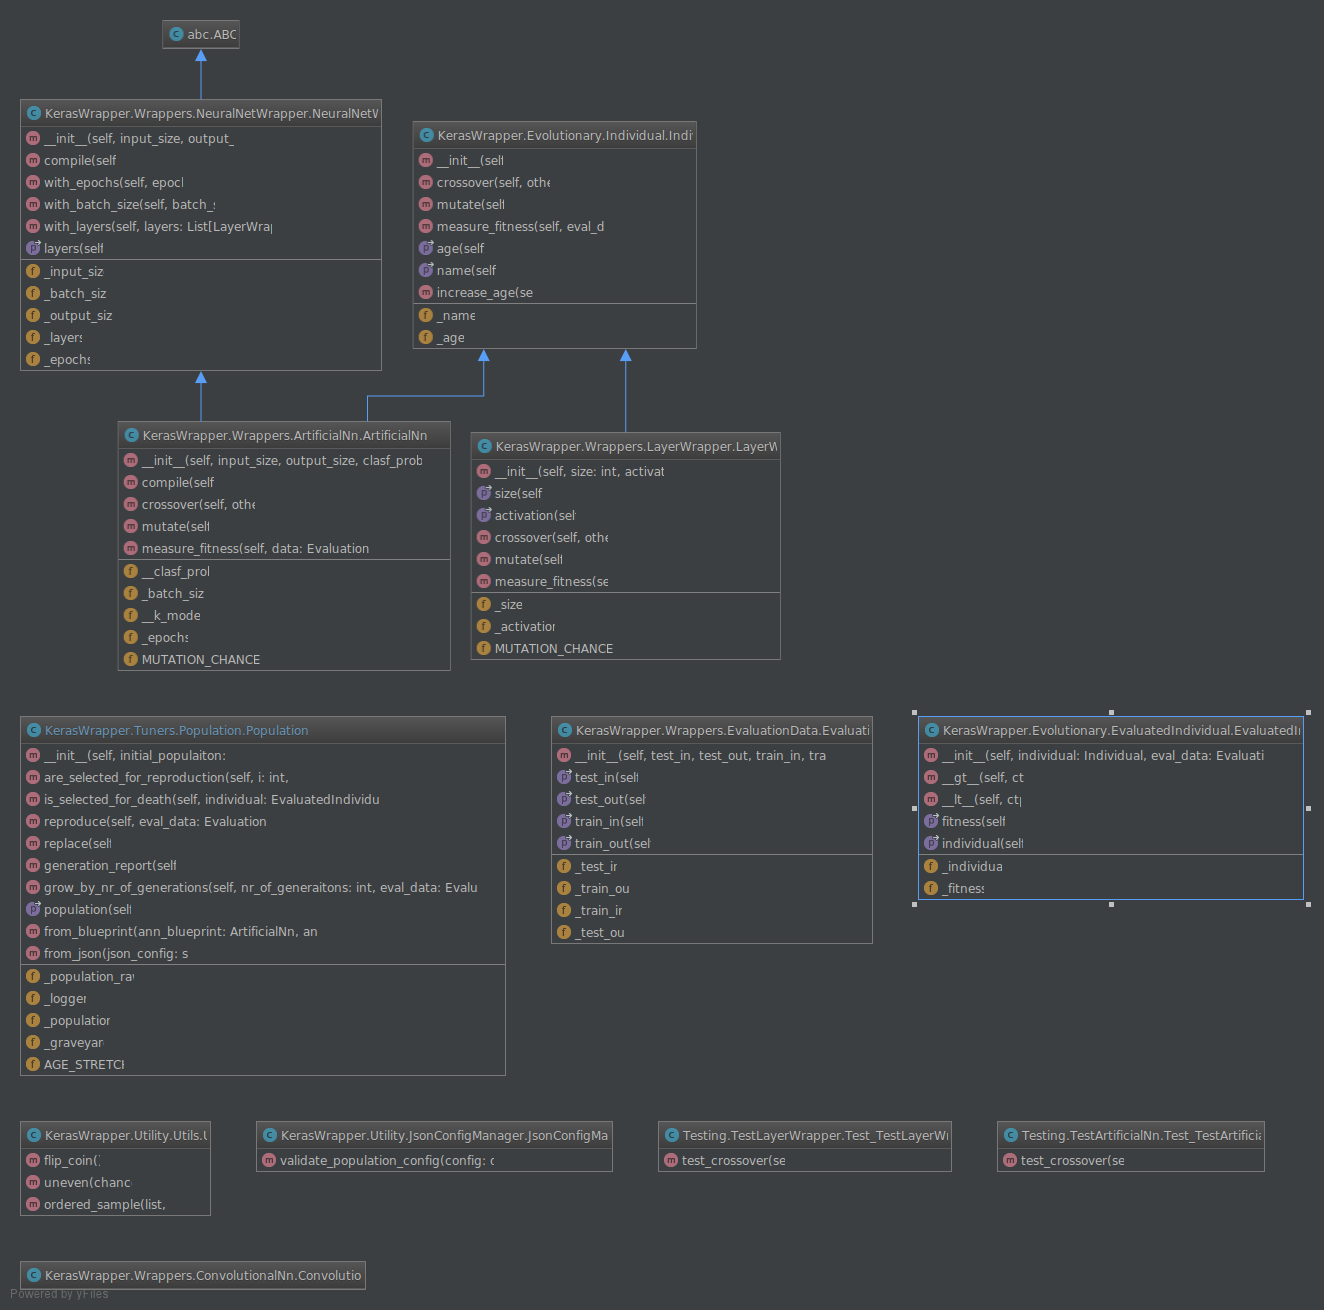
\includegraphics{gfx/BachelorThesis.svg}
\caption{Code architecture}
\end{figure}

    \hypertarget{feasability-and-impact-analysis}{%
\section{4. Feasability and Impact
Analysis}\label{feasability-and-impact-analysis}}

In implementarea algoritmului, s-au folosit mai multe iterații, in care
se testa algoritmul, se observau unele metrici și se luau decizii
ulterioare de implementare.

În găsirea rețelei optime, algoritmul curent consideră hiperparametrii:

Numarul de straturi Marimea unui strat Pentru rețele neuronale s-a
folosit Keras cu back-end Tensor Flow. In implementarea codului s-au
folosit clase care impacheteaza comportamentul din Keras și a căror
utilitate este de a furniza API pentru lucrul cu algoritmii evolutivi.
La bază algoritmii evolutivi folosiți sunt stocastici.

In implementarea inițială avem functia de selectie naturala, care
primeste lista indivizilor sortata descrescator dupa fitness. Se iau
oricare 2 indivizi cu indicele i si j, si se calculeaza sansa lor de a
se reproduce, astfel:

    \[\frac{i \cdot j}{{(n - 1)}^{2}}\]

    S-a implementat si o selecție pentru deces, ce ia in considerare o șansă
calculată proporțional cu fitness-ul individului, precum și vârsta
individului (exprimata in număr de generații). Pentru in individ i,
șansa acestuia de a deceda este calculata astfel:

    \[\frac{a \cdot (1 - \frac{i}{n})}{E}\]

Unde E = speranța de viață și n = numărul total de indivizi

    \hypertarget{metrics-and-testing}{%
\section{Metrics and testing}\label{metrics-and-testing}}

In testarea algoritmului s-a folosit problema clasică de recunoaștere a
caracterelor, cu baza de date MNIST. Indivizii inițiali au fost dați ca
și input.

    \hypertarget{iteration-1}{%
\subsection{Iteration 1}\label{iteration-1}}

\hypertarget{parameters}{%
\subsubsection{Parameters}\label{parameters}}

Life expectancy: 3

\hypertarget{crossover}{%
\subsubsection{Crossover}\label{crossover}}

The crossover of the neural nets was done through the combination of the
hidden layers.

In the case that the crossover parties have different numbers of layers,
a random sampling happenes on the net with more layers. The size of the
sampling is the number of layers of the one with fewer layers (lets call
it A and the counterparty B). The bad thing here is that the genes of A
can be proportionally dominant compared to B, as the layers of B, that
are not included in the sampling, are discarded in the process.

\hypertarget{fitness}{%
\subsubsection{Fitness}\label{fitness}}

The calculation of the fitness is (currently) based only on the accuracy
of the neural network.

\hypertarget{metrics}{%
\subsubsection{Metrics}\label{metrics}}

\begin{itemize}
\tightlist
\item
  Fitness trend

  \includegraphics{gfx/fitness-trend-tne-1.png}
\item
  Generation size

  \includegraphics{gfx/generation-size-tne-1.png}
\end{itemize}

    \hypertarget{iteration-2}{%
\subsection{Iteration 2}\label{iteration-2}}

\hypertarget{parameters}{%
\subsubsection{Parameters}\label{parameters}}

Life expectancy: 1.3

\hypertarget{crossover}{%
\subsubsection{Crossover}\label{crossover}}

Unchanged.

\hypertarget{fitness}{%
\subsubsection{Fitness}\label{fitness}}

Unchanged.

\hypertarget{metrics}{%
\subsubsection{Metrics}\label{metrics}}

\begin{itemize}
\tightlist
\item
  Fitness trend
\end{itemize}

We are now measuring also the maximum fitness of the population

\includegraphics{gfx/fitness-trend-tne-2.png} * Generation size

\begin{figure}
\centering
\includegraphics{gfx/generation-size-tne-2.png}
\caption{title}
\end{figure}

    \hypertarget{observations}{%
\subsection{Observations}\label{observations}}

The main observations made throughout the first two iterations focuses
on weak points of the algorithm:

\begin{itemize}
\item
  One strong weakness is that the populaiton grows quickly.
\item
  This simply doesn't scale, because finding a good solution ot our
  problem, we need to grow a certain amount of generations,
  approximately 10. To grow 4 generations, the program ran for about
  \textasciitilde{}12 hours. The conclusion drew by Generation Size
  metric, this approach doesn't scale. To perform a crossover between
  the genotypes of the generation 4 would take an unreasonably huge
  amount of time.
\item
  Another observations here is that the average fitness converges to a
  value. This means that the genotypes become homogenous. There is not
  enough new genetical material and this will not help us raise the
  maximum fitness either.
\item
  We can see how the maximum fitness increases, but not signtificanlty
  enough to justify the need of such algorithms to find a better
  solution. A significant fitness increase would be achieved by growing
  a larger number of generations.
\item
  The crossover function can be also improved. When performing
  crossover, we can consider all the genes of the individuals, without
  too much domination from one party.
\item
  We can consider other hyperparameters in finding the optimal solution,
  like initial weights and biases.
\item
  The fitness function can also consider the physical running time as a
  quality of a genotype.
\item
  For the following iterations, we will use Tournament Selection for
  selections. This should give us a controllable number of genotypes and
  more generations to grow.
\item
  We can consider trying the same test but for other problems (which can
  also be more complex) and other trainig data sets.
\item
  The input and the train data can be randomly sampled (k-fold)
\end{itemize}

    \hypertarget{bibliography}{%
\section{Bibliography}\label{bibliography}}

{[}1{]}
\href{https://blog.coast.ai/lets-evolve-a-neural-network-with-a-genetic-algorithm-code-included-8809bece164}{Let's
evolve a neural network with a genetic algorithm}

{[}2{]} \href{http://neuralnetworksanddeeplearning.com/chap1.html}{Using
neural nets to recognize handwritten digits}

{[}3{]}
\href{https://www.cs.vu.nl/~gusz/ecbook/Eiben-Smith-Intro2EC-Ch2.pdf}{What
is an Evolutionary Algorithm}

{[}4{]}
\href{https://en.wikipedia.org/wiki/Computational_complexity}{Computational
complexity}


    % Add a bibliography block to the postdoc
    
    
    
    \end{document}
